\clearpage % Rozdziały zaczynamy od nowej strony.

\section{Modifying QEMU source to run PenPointOS}

In this first part I will describe what the JPC emulator is and show the
patches created by prof. Simon Schubiger that allow it to run PenPointOS, as
well as explain why it is not suitable for our goal. Then I will present the
architecture of the QEMU emulator and the reasons it was chosen as the
appropriate solution, and finally I will show how I tried to port the changes
created by prof. Schubiger to the QEMU source.

\subsection{PenPoint for NCR 3125 tablet}

The creators of PenPoint knew that wide adoption would be hard if the barrier
to entry were high. That's why many different versions of PenPoint were created
that could be installed and run on a variety of hardware \cite{carr1991}.

One of those devices was a NCR 3125 \ref{fig:ncr3125} tablet. Although many
tablet-like devices already existed at this point, the System 3125 was the
second pen based computer, the first computer with an external pen
\cite{hohl2014}, and the first pen based computer powerful enough to run
desktop programs like spreadsheet and graphing software \cite{mcdonald2011}.
All of this came at a price - it was one of the most expensive computers
released at the time \cite{hohl2014}. Apart from PenPoint the NCR 3125 also run
MS-DOS with NCR PenOS - proprietary NCR software that allowed for text input
using the stylus, as well as Windows for Pen Computing and GRiD PenRight
\cite{stengel}.

\begin{figure}[!h]
    \centering
    \begin{subfigure}[b]{0.55\linewidth}
        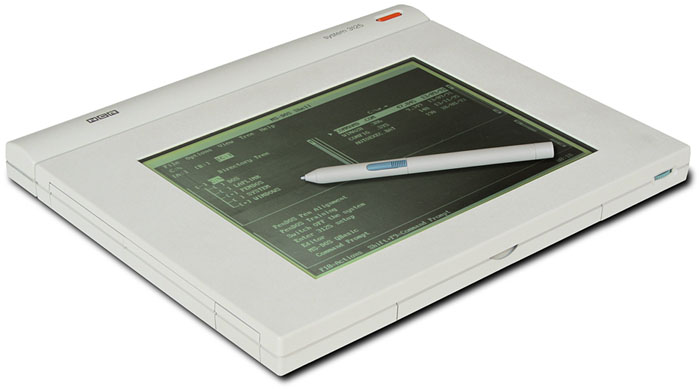
\includegraphics[width=\linewidth]{ncr3125-1.jpg}
        %\caption{NCR 3125}
        %\label{fig:ncr3125-2}
    \end{subfigure}
    \hfill
    \begin{subfigure}[b]{0.35\linewidth}
        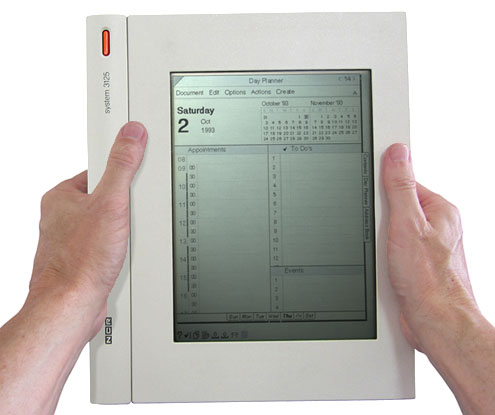
\includegraphics[width=\linewidth]{ncr3125-2.jpg}
        %\caption{NCR 3125}
        %\label{fig:ncr3125-1}
    \end{subfigure}
    \caption{NCR 3125}
    \label{fig:ncr3125}
\end{figure}

The NCR System 3125 was one of the flagship PenPoint computers and its
hardware, apart from the WACOM digitizer, was rather standard x86, thus making
the PenPointOS version for it an appropriate choice for emulation.

\subsection{The JPC emulator}

JPC was created by the University of Oxford's Particle Physics Subdepartment.
Although its github page claims it is fast it was not its main concern. The
advertised features are the flexibility, security and it being cross-platform
given that it is written in 100\% JAVA programming language. These come however
at a cost. The JAVA environment makes it so that JPC can run virtually on any
hardware that JVM is available for, and the memory safety provided by the JVM
as well as sandboxing provide great security. This however comes at a cost, it
will most certainly be much slower than a highly optimised emulator written in
a systems programming language like C or C++. In fact the JPC emulator was too
slow to run PenPoint OS at a speed that would be comfortable for use - the
video showing the operation of PenPoint on JPC on professor's Schubiger channel
had to be sped up to look normal \cite{schubiger2015}.

In the following sections I will show how the JPC emulator works and how it is
designed. Then I will describe the modifications to the source code created by
prof. Simon Schubiger that allow it to run PenPointOS.  JPC was created by the
University of Oxford's Particle Physics Subdepartment. Although its github page
claims it is fast it was not its main concern. The advertised features are the
flexibility, security and it being cross-platform given that it is written in
100\% JAVA programming language. These come however at a cost. The JAVA
environment makes it so that JPC can run virtually on any hardware that JVM is
available for, and the memory safety provided by the JVM as well as sandboxing
provide great security. This however comes at a cost, it will most certainly be
much slower than a highly optimised emulator written in a systems programming
language like C or C++. In fact the JPC emulator was too slow to run PenPoint
OS at a speed that would be comfortable for use - the video showing the
operation of PenPoint on JPC on professor's Schubiger channel had to be sped up
to look normal \cite{schubiger2015}.

In the following sections I will show how the JPC emulator works and how it is
designed. Then I will describe the modifications to the source code created by
prof. Simon Schubiger that allow it to run PenPointOS.

\subsubsection{Architecture of JPC}

The architecture of the JPC emulator is somewhat simple, at least when it comes
to such complex software as a virtual machine. There is a class PC that models
the machine being emulated. It stores all the components and manages them. It
uses a different class implementing the PCConfig interface to provide
configuration. The main function processes the input arguments and based on
them initialises object of the \emph{PC} class. Input arguments control such things
as setting which files are used as harddrives or floppies, as well as choosing
the boot device out of them.

\begin{codeblock}
    \lstinputlisting[
        caption={PC.java},
        language=Java,
        linerange={1109-1110,1156-1170},
    ]{PC.java}
\end{codeblock}

% Fragment kodu źródłowego programu
% \addmargin pozwala na wcięcie kodu od lewej (tu: 8mm).
% Wcięcie służy do tego, aby numery linii nie wystawały poza lewy margines.
% Druga liczba oznacza wcięcie od prawej.
%\begin{minipage}{\linewidth}
%    \begin{addmargin}[8mm]{0mm}
%        \begin{lstlisting}[
%            language=Java,
%            numbers=left,
%            firstnumber=1,
%            %    caption={\emph{Hello world} w HTML},
%            aboveskip=10pt
%            ]
%public static void main(String[] args) {
%    try {
%
%        // ...
%
%        PC pc = new PC(new VirtualClock(), args, Calendar.getInstance());
%        pc.start();
%        try {
%            while (true) {
%                pc.execute();
%            }
%        } finally {
%            pc.stop();
%            LOGGING.log(Level.INFO, "PC Stopped");
%            pc.getProcessor().printState();
%        }
%    } catch (IOException e) {
%        System.err.println("IOError starting PC");
%    }
%}
%        \end{lstlisting}
%    \end{addmargin}
%\end{minipage}

% https://tex.stackexchange.com/a/286097
The responsibility of the configuration provider class is to add all the
necessary objects representing hardware components to the PC class object. It
does so in four steps using methods \emph{configureMotherboard},
\emph{configurePeripherals}, \emph{configurePCI}, and \emph{configureBIOS}. The
meaning of these functions is rather superficial as all of them add instances
of classes implementing \emph{HardwareComponent} interface to the list of all
components managed by the PC class object.


\begin{codeblock}
    \lstinputlisting[
        caption={PC.java},
        language=Java,
        linerange={122-122,141-149},
    ]{PC.java}
\end{codeblock}

%\begin{minipage}{\linewidth}
%    \begin{addmargin}[8mm]{0mm}
%        \begin{lstlisting}[
%            language=Java,
%            numbers=left,
%            firstnumber=1,
%            %    caption={\emph{Hello world} w HTML},
%            aboveskip=10pt
%            ]
%public PC(Clock clock, DriveSet drives, int ramSize, Calendar startTime,
%PCConfig config) throws IOException {
%
%    // ...
%
%    config.configureMotherboard(this, startTime);
%    config.configurePeripherals(this);
%    config.configurePCI(this);
%    config.configureBIOS(this);
%
%    if (!configure()) {
%        throw new IllegalStateException("PC Configuration failed");
%    }
%}
%        \end{lstlisting}
%    \end{addmargin}
%\end{minipage}


The next step is the setting up of all of the managed devices. In the
configuration phase all components are made aware of all the other components
so that they can initialise themselves and establish relations. Here all
devices must connect to the buses, displays and ports as they require. This is
done by repeatedly calling each of the components' method \emph{acceptComponent} to
accept every other component until all components report being fully
initialised.

\begin{codeblock}
    \lstinputlisting[
        caption={PC.java},
        language=Java,
        linerange={447-466},
    ]{PC.java}
\end{codeblock}
            
%\begin{minipage}{\linewidth}
%    \begin{addmargin}[8mm]{0mm}
%        \begin{lstlisting}[
%            language=Java,
%            numbers=left,
%            firstnumber=1,
%            %    caption={\emph{Hello world} w HTML},
%            aboveskip=10pt
%            ]
%private boolean configure() {
%    boolean fullyInitialised;
%    int count = 0;
%    do {
%        fullyInitialised = true;
%        for (HardwareComponent outer : parts) {
%            if (outer.initialised()) {
%                continue;
%            }
%            for (HardwareComponent inner : parts) {
%                outer.acceptComponent(inner);
%            }
%            fullyInitialised &= outer.initialised();
%            if(!fullyInitialised && count > 90)
%            LOGGING.log(Level.WARNING, outer + " not initialized, retry");
%        }
%        count++;
%    } while ((fullyInitialised == false) && (count < 100));
%
%    // ...
%
%        \end{lstlisting}
%    \end{addmargin}
%\end{minipage}

Then also auto-configuration of all PCI devices that is normally done by BIOS
is performed by calling \emph{biosInit} method on all components that are
instances of \emph{PCIBus} class. At this point all the PCI buses are aware of
the PCI connected devices as they were supposed to register themselves in their
\emph{acceptComponent}.

\begin{codeblock}
    \lstinputlisting[
        caption={PC.java},
        language=Java,
        linerange={482-489},
    ]{PC.java}
\end{codeblock}

%\begin{minipage}{\linewidth}
%    \begin{addmargin}[8mm]{0mm}
%        \begin{lstlisting}[
%            language=Java,
%            numbers=left,
%            firstnumber=21,
%            %    caption={\emph{Hello world} w HTML},
%            aboveskip=10pt
%            ]
%    for (HardwareComponent hwc : parts) {
%        if (hwc instanceof PCIBus) {
%            ((PCIBus) hwc).biosInit();
%        }
%    }
%    return true;
%}
%        \end{lstlisting}
%    \end{addmargin}
%\end{minipage}

Inside \emph{biosInit} the bus initialises devices based on their device class,
vendor and device IDs as well as based on if it uses an I/O port or memory
mapped port I/O regions. The device class specifies what type of device it is.
This is checked so that some special initialisation can be done if the device
is a network controller. Vendor ID and Device ID are checked additionally if
needed - these designate the exact brand and model of the device. The
difference between port mapped and memory mapped I/O regions is that the memory
mapped ones use the same bus as memory and use the same set of instructions to
store and load whilst the port mapped use special port bus and adequately use
different instructions for reading and writing than normal memory.

Finally the \emph{main} function calls in an infinite loop the \emph{execute}
method of the \emph{PC} object that executes instructions in processor's
current mode by calling functions of objects representing both processor and
address spaces.

\subsubsection{Implementation of JPC modifications for running PenPointOS}

In this section I will explain what changes have been made by professor
Schubiger in order to make PenPointOS work in the JPC emulator, as well as how
they work. First I will show the overview of what has been changed and then
I will describe in detail three classes representing components of the NCR
System 3125 that were necessary for the purposes of its emulation.

To configure the object of the \emph{PC} class that represents the emulated
machine a class extending \emph{PCConfig} - the \emph{NCR3125} class -  was
created. It also provides the entry point - the \emph{main} function - to this
modified version of JPC. It is pretty much the same as the original, but
slimmed down by removing all of the argument parsing. The \emph{PC} class
object is also initialised using this new \emph{NCR3125} class. The difference
lies in the components that are added in the configuration methods, especially
the components that were specially created for the emulation of the NCR 3125.
Two configuration methods from \emph{PCConfig} are overridden in the
\emph{NCR3125}: \emph{configureBIOS} and \emph{configurePeripherals}. The
\emph{configureBIOS} method is the same as the original - it adds the system
BIOS and VGA BIOS, but conditional adding of sound devices is removed. Changes
to \emph{configurePeripherals} are more substantial.

\begin{codeblock}
    \lstinputlisting[
        caption=NCR3125.java,
        language=Java,
        linerange={48-64},
    ]{NCR3125.java}
\end{codeblock}

%\begin{minipage}{\linewidth}
%    \begin{addmargin}[8mm]{0mm}
%        \begin{lstlisting}[
%            language=Java,
%            numbers=left,
%            firstnumber=1,
%            %    caption={\emph{Hello world} w HTML},
%            aboveskip=10pt
%            ]
%protected void configurePeripherals(PC pc) {
%    pc.add(new Intel82360SL());
%    pc.add(new PIIX3IDEInterface());
%    pc.add(new CLGD6410());
%    pc.add(new Port80(PORT80_CODES));
%    pc.add(new SerialPort(0));
%    pc.add(new SerialPort(1));
%    pc.add(new ParallelPort(0));
%    pc.add(new ParallelPort(1));
%    NCRWacom wacom = new NCRWacom();
%    pc.add(wacom);
%    pc.add(pc.keyboard = new Keyboard(wacom));
%    pc.add(new FloppyController());
%    pc.add(new PCSpeaker());
%}
%        \end{lstlisting}
%    \end{addmargin}
%\end{minipage}

Conditionally adding an ethernet device is removed completely. Third and fourth
\emph{SerialPort}'s are replaced by \emph{ParallelPort} one and two. The
\emph{ParallelPort} class added by professor Schubiger allows for 8 bit reads
and writes to three addresses: \emph{PDATA}, \emph{PSTAT} and \emph{PCON}.
Writes to \emph{PDATA} are logged to the console. There is also a component of
class \emph{Port80} added. This object registers itself with the
\emph{IOPortHandler} with the port 0x80 requested. This port is used for
``power-on self test'' (POST) codes. This class simply logs what kind of test is
performed by writing out code value and summary of the code in the 8 bit write
method. Such a facility could certainly prove useful when debugging, especially
when creating representations of computer components. 

Finally there are also added components representing an Intel 82360SL
processor, Cirrus Logic CLGD6410 VGA controller, and a WACOM digitizer. These
will be described in more detail in the following sections.

\subsubsubsection{The WACOM digitizer}

The \emph{NRCWacom} class representing the WACOM digitizer implements three
interfaces: \emph{IODevice}, \emph{IMouseHandler} and \emph{TimerResponsive}.

The \emph{IMouseHandler} interface requires only one method: \emph{mouseEvent},
which is called to update the state of the pointer. It receives the coordinates
of the pointer as well as the displacement, and also int \emph{buttons} with
bits corresponding to pressed down  buttons set. Particularly if the first bit
is set it means that the pen is firmly against the digitizer and if the second
or third bit is set it means that the button on the pen is pressed.

\begin{codeblock}
    \lstinputlisting[
        caption=NCRWacom.java,
        language=Java,
        linerange={233-239},
    ]{NCRWacom.java}
\end{codeblock}

%\begin{minipage}{\linewidth}
%    \begin{addmargin}[8mm]{0mm}
%        \begin{lstlisting}[
%            language=Java,
%            numbers=left,
%            firstnumber=1,
%            %    caption={\emph{Hello world} w HTML},
%            aboveskip=10pt,
%            columns=fixed,
%            ]
%public void mouseEvent(int x, int y, int z, int dx, int dy, int dz, int buttons)
%{
%    Dimension dim = display.getDisplaySize();
%    this.absx = (int) ((0.87f * x / dim.width)  * NCR_NCRMAXX) + 30;
%    this.absy = (int) ((0.94f * y / dim.height) * NCR_NCRMAXY) + 30;
%    this.buttons = buttons;    
%}
%        \end{lstlisting}
%    \end{addmargin}
%\end{minipage}

Implementing \emph{IMouseHandler} allows the \emph{Keyboard} class to use
\emph{NRCWacom} object as a mouse handler.

The \emph{TimerResponsive} interface is implemented so that a \emph{Timer}
object could call a \emph{callback} method specified by the interface. Inside
the \emph{callback} method the \emph{NCRWacom} fills a ``packet'' of 6 bytes
with status of the digitizer, position of the pen and pressed buttons.

\begin{codeblock}
    \lstinputlisting[
        caption=NCRWacom.java,
        language=Java,
        linerange={241-268},
    ]{NCRWacom.java}
\end{codeblock}

%\begin{minipage}{\linewidth}
%    \begin{addmargin}[8mm]{0mm}
%        \begin{lstlisting}[
%            language=Java,
%            numbers=left,
%            firstnumber=1,
%            %    caption={\emph{Hello world} w HTML},
%            aboveskip=10pt
%            ]
%public void callback() {
%    fillPacket();
%
%    if(streammode != 0) {
%        status |= NCR_DATA_READY;
%        timer.setExpiry(clock.getEmulatedNanos() + interval);
%        irqDevice.setIRQ(irq, 1);
%    }
%}
%
%private void fillPacket() {
%    packet[0] = (byte)(NCR_NCRTAB | NCR_NCRREADY);
%    if     (absx < 0) absx = 0;
%    else if(absx > NCR_NCRMAXX) absx = (int) NCR_NCRMAXX;
%    if     (absy < 0) absy = 0;
%    else if(absy > NCR_NCRMAXY) absx = (int) NCR_NCRMAXY;
%
%    packet[1] = (byte)(absx >> 8);
%    packet[2] = (byte)absx;
%    packet[3] = (byte)(absy >> 8);
%    packet[4] = (byte)absy;
%    packet[5] = 0;
%    if((buttons & 0x1) != 0) packet[5] |= NCR_NCRPENZ;
%    if((buttons & 0x6) != 0) packet[5] |= NCR_NCRBUTTON;
%}
%        \end{lstlisting}
%    \end{addmargin}
%\end{minipage}

This ``packet'' is then read by 8 bit I/O reads from the data register.

\begin{codeblock}
    \lstinputlisting[
        caption=NCRWacom.java,
        language=Java,
        linerange={148-171},
    ]{NCRWacom.java}
\end{codeblock}

%\begin{minipage}{\linewidth}
%    \begin{addmargin}[8mm]{0mm}
%        \begin{lstlisting}[
%            language=Java,
%            numbers=left,
%            firstnumber=1,
%            %    caption={\emph{Hello world} w HTML},
%            aboveskip=10pt
%            ]
%public int ioPortRead8(int address) {
%    switch(address) {
%        case NCR_DATA_REG:
%        int result = 0;
%        if(echobackptr >= 0) {
%            result = echoback[echobackptr++];
%            if(echobackptr >= echoback.length) {
%                echobackptr = -1;
%            }
%        } else {
%            result = packet[packetptr++];
%            if(packetptr >= packet.length) {
%                packetptr = 0;
%                status &= ~NCR_DATA_READY;
%                irqDevice.setIRQ(irq, 0);
%            }
%        }
%        return result;
%        case NCR_STATUS_REG:
%        return status;
%    }
%    return super.ioPortRead8(address);
%}
%        \end{lstlisting}
%    \end{addmargin}
%\end{minipage}

The \emph{Timer} object is created from the \emph{Clock} object. The
\emph{Clock} object along with \emph{InterruptController} and
\emph{IDisplayAdapter} are obtained and set during the component initialisation
stage performed by the \emph{PC} object by calling \emph{acceptComponent}
method. The \emph{IDisplayAdapter} is used to get dimensions of the display in
the \emph{mouseEvent} method, and the \emph{InterruptController} is used to
raise interrupt when the ``packet'' is filled and unset it when the ``packet''
is wholly read. Apart from these objects, an instance of \emph{IOPortHandler} is
used to register \emph{NCRWacom} as capable for I/O using
\emph{registerIOPortCapable}. What it means will be explained in the next
paragraph.

Finally the \emph{IODevice} interface is the most important piece, as it
provides all of the methods used for I/O, and this is where all of the changing
the state of the device and most of the logic, as well as reporting of the
state will happen.

\begin{codeblock}
    \lstinputlisting[
        caption=IODevice.java,
        language=Java,
        firstline=3,
    ]{IODevice.java}
\end{codeblock}

%\begin{minipage}{\linewidth}
%    \begin{addmargin}[8mm]{0mm}
%        \begin{lstlisting}[
%            language=Java,
%            numbers=left,
%            firstnumber=1,
%            %    caption={\emph{Hello world} w HTML},
%            aboveskip=10pt
%            ]
%public interface IODevice {
%
%    public void ioPortWrite8(int address, int data);
%
%    public void ioPortWrite16(int address, int data);
%
%    public void ioPortWrite32(int address, int data);
%
%    public int ioPortRead8(int address);
%
%    public int ioPortRead16(int address);
%
%    public int ioPortRead32(int address);
%
%    public int[] ioPortsRequested();
%}
%        \end{lstlisting}
%    \end{addmargin}
%\end{minipage}

The \emph{NCRWacom} overrides three methods used for I/O. To let the
\emph{IOPortHandler} object know what ports are needed, \emph{ioPortsRequested}
method is used. Apart from that methods for 8 bit read and write are provided:
\emph{ioPortRead8} and \emph{ioPortWrite8}. The \emph{ioPortRead8} allows
reading from two addresses: the status register returns if the device is ready
for command (always set), and if data - the ``packet'' is ready; the data
register contains either a set of predefined values if it was not previously
read or if \emph{NCR\_ECHOBACK} command was issued, or else it contains
consecutive bytes of the ``packet''. Otherwise implementation of
\emph{ioPortRead8} from the superclass - \emph{AbstractHardwareComponent} is
called which just prints to console.

The \emph{ioPortWrite8} writes to either data register which is a noop or to
command register, otherwise again the write is delegated to the superclass
which does a print to console.

\begin{codeblock}
    \lstinputlisting[
        caption={},
        language=Java,
        linerange={99-104},
    ]{NCRWacom.java}
    \dots
    \lstinputlisting[
        caption=NCRWacom.java,
        language=Java,
        linerange={142-146},
    ]{NCRWacom.java}
\end{codeblock}

%\begin{minipage}{\linewidth}
%    \begin{addmargin}[8mm]{0mm}
%        \begin{lstlisting}[
%            language=Java,
%            numbers=left,
%            firstnumber=1,
%            %    caption={\emph{Hello world} w HTML},
%            aboveskip=10pt
%            ]
%public void ioPortWrite8(int address, int data) {
%    switch(address) {
%    case NCR_DATA_REG:
%        break;
%    case NCR_COMMAND_REG:
%        // ...
%        \end{lstlisting}
%        \begin{lstlisting}[
%            language=Java,
%            numbers=left,
%            firstnumber=42,
%            %    caption={\emph{Hello world} w HTML},
%            aboveskip=10pt
%            ]
%        break;
%    default:
%        super.ioPortWrite8(address, data);
%    }
%}
%        \end{lstlisting}
%    \end{addmargin}
%\end{minipage}

There are a few possible commands that can be written to the command register.
Commands \emph{NCR\_STREAMSTOP} and \emph{{NCR\_RESET}} turn off stream mode.
Stream mode makes it so that the callback invoked by the \emph{Timer} does not
set the next time it is called and does not raise the interrupt.

\begin{codeblock}
    \lstinputlisting[
        caption=NCRWacom.java,
        language=Java,
        linerange={104-111},
    ]{NCRWacom.java}
\end{codeblock}

%\begin{minipage}{\linewidth}
%    \begin{addmargin}[8mm]{0mm}
%        \begin{lstlisting}[
%            language=Java,
%            numbers=left,
%            firstnumber=6,
%            %    caption={\emph{Hello world} w HTML},
%            aboveskip=10pt
%            ]
%    case NCR_COMMAND_REG:
%        switch(data) {
%        case NCR_STREAMSTOP:
%            streammode = 0;
%            break;
%        case NCR_RESET:
%            streammode = 0;
%            break;
%
%        \end{lstlisting}
%    \end{addmargin}
%\end{minipage}

The \emph{NCR\_ECHOBACK} command makes it so the next \emph{ioPortRead}s from
the data register will return values from the predefined ``echo''.

\begin{codeblock}
    \lstinputlisting[
        caption=NCRWacom.java,
        language=Java,
        linerange={112-114},
    ]{NCRWacom.java}
\end{codeblock}

The \emph{NCR\_REQUEST} updates the ``packet'' and sets the data ready bit in
status.

\begin{codeblock}
    \lstinputlisting[
        caption=NCRWacom.java,
        language=Java,
        linerange={115-119},
    ]{NCRWacom.java}
\end{codeblock}

There are also 7 \emph{NCR\_STREAM*} commands that turn on the stream mode and
change interval at which the \emph{Timer} callbacks are set to occur.

\begin{codeblock}
    \lstinputlisting[
        caption=NCRWacom.java,
        language=Java,
        linerange={120-138},
    ]{NCRWacom.java}
\end{codeblock}

\subsubsubsection{The Intel 82360 SL processor}

The interesting thing about the \emph{Intel82360SL} class is that it does not
implement all of the functionality of a processor. In fact it is very simple
and short - all of its logic is contained in 8 bit and 16 bit I/O port read and
write functions. Instead it is added as a component in addition to the default
\emph{Processor} class used by \emph{PC} class.

The 8 bit write function - \emph{ioPortWrite8} - if called with a write to
address \emph{CFGSTAT} with value of 0 increases value of \emph{unlock} by 1.
This value of \emph{lock} guards writes to several other addresses. It holds
whether configuration space was unlocked and whether the selected unit is
enabled. 

\begin{codeblock}
    \lstinputlisting[
        caption={},
        language=Java,
        linerange={171-173},
    ]{Intel82360SL.java}
    \dots
    \lstinputlisting[
        caption={},
        language=Java,
        linerange={184-187},
    ]{Intel82360SL.java}
    \dots
    \lstinputlisting[
        caption=Intel82360SL.java,
        language=Java,
        linerange={198-199},
    ]{Intel82360SL.java}
\end{codeblock}

Then a 8 bit write to \emph{CPUPWRMODE} when \emph{unlock} is equal to 1 -  so
when configuration space is unlocked - with a value of ``0x80'', that is with all
but most significant bit set, increases value of \emph{unlock} again, and with
that enables selected unit. When the \emph{unlock} value is greater than 2 the
written value is stored in \emph{cpupwrmode}.

\begin{codeblock}
    \lstinputlisting[
        caption=Intel82360SL.java,
        language=Java,
        linerange={174-179},
    ]{Intel82360SL.java}
\end{codeblock}

Similarly when configuration space is both unlocked and selected unit is
enabled 8 bit writes to \emph{CFGINDEX} store the value written to \emph{idx}
which is later used in case of 8 bit write to \emph{CFGDATA} which stores write
data into \emph{regs} under previously selected \emph{idx}.

\begin{codeblock}
    \lstinputlisting[
        caption=Intel82360SL.java,
        language=Java,
        linerange={180-183,188-191},
    ]{Intel82360SL.java}
\end{codeblock}

In the default case the write is delegated to the 16 bit version of the
function by converting the address to 16 bit version through making the address
even by zeroing the lowest bit, performing a 16 bit read from the address to
obtain the other 8 bits, and performing 16 bit write with combined data of the
original write with the value of the other byte. This results in calling the
superclass counterpart of this method which simply performs printing to
console, since the only address handled by the 16 bit write method is
\emph{CPUPWRMODE} which is also covered by the 8 bit version.

The 8 bit read function allows to obtain value of \emph{cfgtstat} by reading
from address \emph{CFGSTAT}. This variable is never used nor initialised so it
seems like to be a mistake. Reading from address \emph{CFGDATA} bears value
stored in \emph{regs} at index \emph{idx}. Four addresses 0xFFF9, 0xFFFB,
0xFFFD, and 0xFFFF always contain 0. For all other addresses the read is
delegated to the 16 bit version of the function with aligning the address to 16
bits and masking and shifting the result to convert it back to 8 bits.

\begin{codeblock}
    \lstinputlisting[
        caption=Intel82360SL.java,
        language=Java,
        linerange={201-217},
    ]{Intel82360SL.java}
\end{codeblock}

The \emph{ioPortWrite16} method allows for writing to \emph{CPUPWRMODE}
address. Otherwise it reverts to using the superclass implementation which just
logs the write. Analogically to the 8 bit version increases the \emph{unlock}
and updates the value of \emph{cpupwrmode} with data written, but it adds to
\emph{unlock} when its value is equal to 2 instead of 1 like the
\emph{ioPortWrite8} does.

The function \emph{ioPortRead16} allows for reads from \emph{PPCONFIG} address
or otherwise prints out information about the read by referring to the same
method in the base class.

\begin{codeblock}
    \lstinputlisting[
        caption=Intel82360SL.java,
        language=Java,
        linerange={149-169},
    ]{Intel82360SL.java}
\end{codeblock}

\subsubsubsection{The Cirrus Logic CLGD6410 VGA controller}

The implementation file for the CLGD6410 VGA controller is rather big,
especially in comparison to the other source modifications provided by
professor Schubiger, spanning just under 3000 lines of code. But it turns out
that a great deal of it is the same as the code for the originally provided VGA
card with minor modifications.

The \emph{CLGD6410} class is pretty much a copy of the \emph{VGACard} class
with additional functionality provided by the class \emph{DefaultVGACard}
included as well. The \emph{DefaultVGACard} normally extends the \emph{VGACard}
class with some utility functions like getting display dimensions, saving
screenshots or adding monitors. The object of that class is then normally used
as one of the components of a PC. Apart from that all of the PCI and interrupt
request code is removed, VRAM size is changed, and new addresses for I/O are
added, as well as a bunch of requested I/O ports are used in addition to the
ones in the default implementation. The VGA RAM size is changed from 16M to
256K. Finally there are added new addresses for graphics, sequencer, attribute,
and crt registers to write, as well as new possible values that could be
written.

\subsubsection{Building and running JPC with the patch}

Unfortunately I failed to build and run PenPointOS with this modified version
myself. The original source code is really old, and targets an outdated Java
version, that my installation would refuse to compile. But even after changing
the target version, fixing some hardcoded paths that were used for resources,
and updating some parts of the code to adhere to the newer version of Java the
program crashed. Despite this I still planned to port these changes to the QEMU
emulator by reading and understanding the logic and intent behind the changes
in the patch.

\subsection{The QEMU hypervisor}

The QEMU emulator is a much more complex piece of software than the JPC
emulator. It has multiple target host and guest architectures - that is it is
possible for QEMU to run on many differing types of machines, as well as it is
possible to emulate different computer types. QEMU also offers utility tools
used for emulation purposes like creation of disk images, as well as provides
programs both for system emulation and for user emulation - meaning an emulator
for a whole system or or an emulator for a single executable that was compiled
for a different architecture. What is more, QEMU is not only an emulator but it
is actually a hypervisor. In this case it means that the emulation is not
necessarily done in software only but is also ``hardware accelerated'' in some
way. QEMU has the ability to run guest instructions directly on host hardware
with tiny or negligible overhead.  This can be achieved by using special host
instructions meant for virtualization, and trapping signals. QEMU is also
written in the C programming language which by its nature is fast, and it also
allows for careful optimization by hand whether by using handwritten assembly or
by using compiler intrinsics. What is more, QEMU is a free libre open source
software that is actively developed by the community, and many big firms are
interested in its improvement. All of that makes QEMU's performance unbeatable,
but also makes for a plethora of other problems and complications.

Being free and open source software under the GPL2 licence, written in C and
with a thriving community makes it great for contributions. Although many open
source projects neglect creating and maintaining documentation, and in case of
projects that often require expert knowledge like that one such behaviour has
a byproduct of filtering out people that would not be adequately equipped to
work on them, QEMU has a rather good documentation even if sometimes lacking or
outdated, at least in comparison to others similarly specialised projects. This
combined with the immense performance that QEMU offers makes it suitable for
building modifications that would allow it to run PenPoint OS on modern
hardware with necessary speed for comfortable use.

In the following sections I will explain how QEMU operates, show the process of
creating a new device in the QEMU source tree, and explain how QEMU's build
system works.

\subsubsection{Operation of QEMU}

In order to support many target host and guest architectures it is necessary to
decouple implementation of one from the other - perform some sort of ``strength
reduction'' - instead of creating a combination of all possible pairs of host
and guest it is only required to provide a sum by using an universal
intermediate step. This way the host backend has to only translate host
instructions to one special set of instructions and from there guest frontend
only has to convert from one special set of instructions. Doing it this way has
also the added benefit of adding a new host, new guest or modifying
implementation of existing one without having to change anything else. This is
what Tiny Code Generator (TCG) does. As it turns out this also helps with
performance optimization.

A basic mode of operation for translating opcodes in an intermediate manner
would be to fetch and convert the instruction. Then some sort of code
initialising the execution environment would be performed, the instruction would
be run, and finally a cleanup would occur. QEMU in order to increase the speed
of execution fetches multiple instructions at a time for translation.  These
portions of instructions are then converted to what is called a Translation
Block (TB). A Translation Block is created when a branch instruction is
encountered or the internal state of the processor that would affect the
execution is changed. That means that TB's have only a single exit point. It is
not possible to jump to the middle of a Translation Block. In such a situation
a new TB would have to be created. This means that one Translation Block can
have only one entry and one exit point. After a TB is created it is inserted
into cache. That way next time QEMU needs to execute an instruction it can check
if the corresponding Translation Block was already ready, and completely skip
that stage if possible. In order to execute a TB the execution environment must
be set up. This is the ``prologue''. After the TB finishes a cleanup must be
performed. This is the ``epilogue''. Because these ``prologues'' and
``epilogues'' can be quite costly performance wise QEMU can chain multiple TBs
together without ``prologues'' and ``epilogues'' in between. QEMU also performs
several optimizations on the Translation Blocks such as dead code elimination
\cite{qemu2022}.

\subsubsection{Adding a device code to the QEMU source tree}

QEMU uses an object oriented approach for defining new devices which would be
great if it wasn't for the fact that QEMU is written in C programming language.
What it means is that all of the inheritance and method overriding must be done
by hand by the programmer. But that's not all. For this to work all of that has
to be passed around by either opaque void pointers or pointers to the base
class and stringly type-checked at runtime. Unfortunately there does not really
exist any official documentation for creating new devices apart from a general
QEMU Object Model (QOM) overview that only describes the process of registering
a new type. Best we can do is to analyse source code of the educational device
that exists in QEMU repository or read through comments of many source header
files located in different places associated with device creation.

In order for the device to be available to QEMU it has to be registered. The
way to do this is to create an object that describes the type of said device.
It contains the parent class as well as information on how both the object
representing class of the device, and object representing instance of the
device should be instantiated. Inside the class initialization function all of
the additional data needed to create an instance of the class has to be set, as
well as all of the information required by the parent class. The instance setup
function is responsible for initialising the object that represents the state
of the device. Additionally some classes of devices, like PCI devices, have
their own required functions used for initialization, cleanup or other. The
last step to making the newly created device available to QEMU is adding the
source file to the build system, which is rather complicated to say the least,
so that it is compiled and linked with the desired binary.

In the following subsections I will present an extremely simple example device,
and describe a little more complex educational device that exists within QEMU
source code. In a subsequent section I will show how the QEMU build system
works and how to add a device to be compiled.

\subsubsubsection{Simple example device implementation}

First thing to do when creating a new device in QEMU is to create structs that
will represent the class and the state of an instance of the device. The object
representing the class should hold all of the methods - the virtual  table, as
well as all of the data associated with the class. The instance struct ought to
contain the internal state of the device. As opposed to the instance struct
objects of which are created for every device the class struct is created only
once for every device type. To declare the new object type a macro
\emph{OBJECT\_DECLARE\_TYPE} is used with the instance struct, class struct,
and the name of the module. This macro provides the standard type casting
functions and registers the instance struct to be used with \emph{g\_autoptr}
so that it is cleaned up properly. The \emph{TYPE\_TEST} string will be used to
specify this device on the QEMU command line, and although not directly
specified it is used for type checking in the casting functions defined by
\emph{OBJECT\_DECLARE\_TYPE}.

\begin{codeblock}
    \lstinputlisting[
        caption=test-device.c,
        language=C++,
        linerange={8-18},
    ]{test-device.c}
\end{codeblock}

The next step is to define the methods and the device logic. Because this
device does not do anything, only the basic functions for the class and instance
initialization and for instance cleanup are defined.

\begin{codeblock}
    \lstinputlisting[
        caption=test-device.c,
        language=C++,
        linerange={20-30},
    ]{test-device.c}
\end{codeblock}

The last step is to register the newly created device for use. This is done by
creating a variable of type \emph{TypeInfo} that contains all the necessary
information about the type for its instantiation: the sizes and constructors
for the instance and class objects, as well as the base class and name used to
specify this device on command line. A function that will register this type by
passing this variable as argument has to be defined. And finally using a macro
\emph{type\_init} this function is added to the list of functions to be run at
startup so that it is called before main.

\begin{codeblock}
    \lstinputlisting[
        caption=test-device.c,
        language=C++,
        linerange={38-53},
    ]{test-device.c}
\end{codeblock}

\subsubsubsection{The QEMU edu device}

The educational device was created for use in the linux kernel course at
Masaryk University. It is a simple PCI device that can respond to reads and
writes, generates interrupts and performs Direct Memory Access (DMA).

Similarly to the example device from the previous section it defines the
instance struct and uses a macro to generate the casting functions. It does not
define any class struct because it uses \emph{PCIDeviceClass} without any
modifications. For the same reason \emph{DECLARE\_INSTANCE\_CHECKER} macro can
be used - the machinery for \emph{PCIDeviceClass} was already defined. 

\begin{codeblock}
    \lstinputlisting[
        caption={},
        language=C++,
        linerange={47-49},
    ]{edu.c}
    \dots
    \lstinputlisting[
        caption=edu.c,
        language=C++,
        linerange={78-78},
    ]{edu.c}
\end{codeblock}

The \emph{TypeInfo} variable used for registering the type also has field
\emph{interfaces} initialised. It is a list of used interfaces and in this case
it contains only \emph{INTERFACE\_CONVENTIONAL\_PCI\_DEVICE}.

\begin{codeblock}
    \lstinputlisting[
        caption=edu.c,
        language=C++,
        linerange={425-442},
    ]{edu.c}
\end{codeblock}

In the class initialisation function \emph{edu\_class\_init} additional PCI
specific information has to be set: the PCI class, vendor and device IDs, as
well as two PCI methods: \emph{realize} and \emph{exit}. The instance
initialisation function \emph{edu\_instance\_init} simply sets the DMA mask and
marks it as a property that can be changed on the command line.

\begin{codeblock}
    \lstinputlisting[
        caption=edu.c,
        language=C++,
        linerange={402-423},
    ]{edu.c}
\end{codeblock}

The \emph{realize} PCI function is set to \emph{pci\_edu\_realize}. It sets up
the interrupts, a timer with a callback that will be used for DMA, creates
a thread that will be used for calculating a factorial and initialises a mutex
and condition variable that it will use for synchronisation, finally it
initialises a memory region for I/O.

\begin{codeblock}
    \lstinputlisting[
        caption=edu.c,
        language=C++,
        linerange={362-384},
    ]{edu.c}
\end{codeblock}

The \emph{pci\_edu\_uninit} function is used for PCI \emph{exit}. It makes the
computation thread break out of an infinite loop and joins it, destroys the
mutex, conditional variable and timer, and initialises the MSI interrupt.

\begin{codeblock}
    \lstinputlisting[
        caption=edu.c,
        language=C,
        linerange={385-400},
    ]{edu.c}
\end{codeblock}

The memory mapped I/O read function \emph{edu\_mmio\_read} checks first if the
read size is correct or else it returns early.

\begin{codeblock}
    \lstinputlisting[
        caption=edu.c,
        language=C,
        linerange={189-200},
    ]{edu.c}
\end{codeblock}

\noindent
Then depending on the address it allows to read a register containing an identification value,

\begin{codeblock}
    \lstinputlisting[
        caption=edu.c,
        language=C,
        linerange={202-205},
    ]{edu.c}
\end{codeblock}

\noindent
the computed value of factorial,

\begin{codeblock}
    \lstinputlisting[
        caption=edu.c,
        language=C,
        linerange={209-213},
    ]{edu.c}
\end{codeblock}

\noindent
the status register and interrupt request status register,

\begin{codeblock}
    \lstinputlisting[
        caption=edu.c,
        language=C,
        linerange={214-219},
    ]{edu.c}
\end{codeblock}

\noindent
as well as addresses used for DMA, DMA transfer count and DMA command register.

\begin{codeblock}
    \lstinputlisting[
        caption=edu.c,
        language=C,
        linerange={220-232},
    ]{edu.c}
\end{codeblock}

\noindent
It also allows to read a register providing liveness check by storing bit inverse of value written to it.

\begin{codeblock}
    \lstinputlisting[
        caption=edu.c,
        language=C,
        linerange={206-208},
    ]{edu.c}
\end{codeblock}

The \emph{edu\_mmio\_write} function providing memory mapped I/O writes
similarly to the read function checks first whether the write size is correct.

\begin{codeblock}
    \lstinputlisting[
        caption=edu.c,
        language=C,
        linerange={237-248},
    ]{edu.c}
\end{codeblock}

\noindent
Writing to the factorial register sets the value of which factorial should be
computed next under the condition that a computation is not taking place
already.

\begin{codeblock}
    \lstinputlisting[
        caption=edu.c,
        language=C,
        linerange={250-250,254-257,261-266},
    ]{edu.c}
\end{codeblock}

\noindent
The status register allows to control whether an interrupt should be raised
after finishing factorial computation. Then there are two registers with which
interrupt requests can be raised and acknowledged.

\begin{codeblock}
    \lstinputlisting[
        caption=edu.c,
        language=C,
        linerange={267-279},
    ]{edu.c}
\end{codeblock}

\noindent
Finally there are four registers that are used to change DMA settings: the
source and destination addresses, the transfer count and the command.

\begin{codeblock}
    \lstinputlisting[
        caption=edu.c,
        language=C,
        linerange={280-295},
    ]{edu.c}
\end{codeblock}

The thread whose task is to compute the value of a factorial consists of an
infinite loop. Inside the loop it waits until it is either commanded to finish
or a computation of a new value is requested by a MMIO write to the factorial
register.

\begin{codeblock}
    \lstinputlisting[
        caption=edu.c,
        language=C,
        linerange={317-328},
    ]{edu.c}
\end{codeblock}

\noindent
If it is commanded to finish it breaks out of the infinite loop.

\begin{codeblock}
    \lstinputlisting[
        caption=edu.c,
        language=C,
        linerange={330-333},
    ]{edu.c}
\end{codeblock}

\noindent
Otherwise it reads the requested value to compute factorial of and enters
a computation loop.

\begin{codeblock}
    \lstinputlisting[
        caption=edu.c,
        language=C,
        linerange={335-340},
    ]{edu.c}
\end{codeblock}

\noindent
After that is done the value in the factorial register is updated. If an
interrupt request was set using the status register to be issued after
computation of factorial was completed it is done so now.

\begin{codeblock}
    \lstinputlisting[
        caption=edu.c,
        language=C,
        linerange={347-360},
    ]{edu.c}
\end{codeblock}

There is also support for Direct Memory Access. Whenever a value is written to
the DMA command register a timer is set to run the \emph{edu\_dma\_timer}
callback after 100 nanoseconds.

\begin{codeblock}
    \lstinputlisting[
        caption={},
        language=C,
        linerange={289-294},
    ]{edu.c}
    \dots
    \lstinputlisting[
        caption={},
        language=C,
        linerange={171-173},
    ]{edu.c}
    \dots
    \lstinputlisting[
        caption=edu.c
        language=C,
        linerange={184-187},
    ]{edu.c}
\end{codeblock}

The \emph{edu\_dma\_timer} function performs either read or write based on the
contents of the DMA command register from the address set by the DMA source
register to the address set by the DMA destination register. Then an interrupt
request is raised based again on the value of the DMA command register.

\begin{codeblock}
    \lstinputlisting[
        caption=edu.c,
        language=C,
        linerange={138-169},
    ]{edu.c}
\end{codeblock}

\subsubsection{QEMU build system}

The QEMU build system is extremely convoluted. It probably started as something
that had to support a large number of targets, architectures and configuration
options but was reasonable, but then it grew and after years it became
unrecognisable. The build process is done in three stages but to the user it
takes two steps. It uses a meta build system, two build systems and a configure
script underneath. The first stage is the configure script. It is a standard
script written in POSIX SH. It is used to determine the local build
characteristics like what kind of tools and libraries are available. The second
stage uses the Meson meta build system. It also determines the local build
characteristics. Meson also processes \emph{Kconfig} and \emph{*.mak} files
that describe the dependencies among various features and subsystems. The
\emph{Kconfig} files use almost the same language as the linux kernel
\emph{Kconfig} files but only so slightly different. The output of the Meson
stage are \emph{build.ninja} files but the ninja build tool is not used.
Instead the files are used to synthesise rules for Make. The final stage and
also the second step for the user is to run Make with the rules created from
the ninja file \cite{qemu2022}.

In order to make the simple example device defined before available to QEMU at
runtime it is only necessary to create a new entry in the \emph{Kconfig} file
in the parent directory of where the source file for the device is located. In
this case a simple \emph{default y} states that the configuration option this
entry denotes will always be true.

\begin{codeblock}
    \lstinputlisting[
        caption=Kconfig,
        language=C,
        linerange={50-52},
    ]{Kconfig}
\end{codeblock}

\noindent
We can do it this way because the device does not depend on anything, does not
provide anything, and frankly does not do anything. Had it more complicated
dependency relationships one would have to use the \emph{Kconfig} to specify
dependencies, reverse dependencies, default and conditionally default values.
The next step is to modify the \emph{meson.build} file to add the new source
file to the appropriate sourceset if the configuration option created in the
\emph{Kconfig} file is set.

\begin{codeblock}
    \lstinputlisting[
        caption=meson.build,
        language=Python,
        linerange={20-20},
    ]{meson.build}
\end{codeblock}

\noindent
Now after the changes to the \emph{Kconfig} and \emph{meson.build} files the
newly created device can be specified on the command line. The output shows
that a class is initialised  once but an instance is created for each device
specified \ref{fig:qemu-test-device-output}.

%\begin{figure}[!h]
\begin{figure}[H]
    \centering
    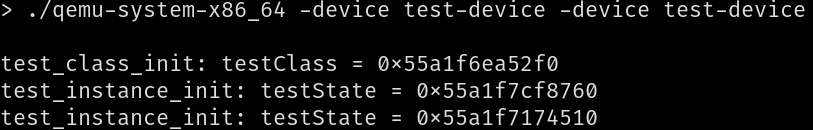
\includegraphics[width=0.9\linewidth]{qemu-test-device-output.png}
    \caption{QEMU test device output}
    \label{fig:qemu-test-device-output}
\end{figure}

\subsection{Conclusion}

In the end the issues with the modified JPC emulator, the steep learning curve
for QEMU development and a possibility that debugging something or
understanding why something does not work could prove simply impossible for me
or require knowledge that could take years to obtain, especially if the only
symptom is that the system does not boot, made me abandon QEMU as a platform to
use. This was also motivated by the fact that a more straightforward solution,
which will be discussed in the next chapter,  presented itself.

